\section{Proposed Methods}
\label{sec:methods}

\subsection{The DeepLab-CRF Model for Semantic Image Segmentation}

Our starting point is the recently proposed DeepLab model for semantic
image segmentation of \citet{chen2014semantic}, illustrated in
Figure~\ref{fig:model_test}. This model applies a deep CNN to an image
in a sliding window fashion to generate score maps for each pixel
location $i = 1, \dots, N$
\begin{equation}
  \label{eq:scores}
  f_i(x_i; \thetav) \,,
  \quad \mathrm{with} \quad
  P_i(x_i; \thetav) \propto \exp \left( f_i(x_i; \thetav) \right)
\end{equation}
where $x_i \in \mathcal{L}$ is the $i$-th pixel's assignment to the
discrete candidate semantic label set $\mathcal{L}$, $\thetav$ is the
vector of CNN model parameters, and normalization ensures that
$\sum_{x_i \in  \mathcal{L}} P_i(x_i; \thetav) = 1$ for every pixel
$i$. Computation sharing in the convolutional layers by means of the
hole algorithm and careful network crafting as detailed in
\citet{chen2014semantic} make the method computationally efficient.

Score map post-processing by means of a fully-connected CRF (Dense CRF)
\cite{krahenbuhl2011efficient} significantly improves segmentation
performance near object boundaries. Specifically,
\citet{chen2014semantic} integrate into their system the fully
connected CRF model of \citet{krahenbuhl2011efficient}.
The model employs the energy function
\begin{align}
  E(\boldsymbol{x}) = \sum_i f_i(x_i) + \sum_{ij} g_{ij}(x_i, x_j)
\end{align}
where $x_i$ is the $i$-th pixel's label assignment. The
additional pairwise potential $g_{ij}(x_i, x_j) =
\mu(x_i,x_j)\sum_{m=1}^{K} w_m \cdot k_m(\boldsymbol{y}_i,
\boldsymbol{y}_j)$, where $\mu(x_i,x_j)=1 \text{ if } x_i \neq x_j$,
and zero otherwise (\ie, Potts Model). There is one such term for
each pair of pixels $i$ and $j$ in the image no matter how far from
each other they lie. Each $k_m$ is the Gaussian kernel depends on features
(denoted as $\boldsymbol{y}$) extracted for pixel $i$ and $j$ and is
weighted by parameter $w_m$. \citet{chen2014semantic} employ bilateral
position and color terms, specifically:
\begin{multline}
  \label{eq:fully_crf}
  w_1 \exp \Big(-\frac{||p_i-p_j||^2}{2\sigma_\alpha^2}
  -\frac{||I_i-I_j||^2}{2\sigma_\beta^2} \Big)\\
  + w_2 \exp \Big(-\frac{||p_i-p_j||^2}{2\sigma_\gamma^2}\Big)
\end{multline}
where the first kernel depends on both pixel positions (denoted as $p$) and
pixel color intensities (denoted as $I$), and the second kernel only depends
on pixel positions. The hyper parameters $\sigma_\alpha$, $\sigma_\beta$ and
$\sigma_\gamma$ control the ``scale'' of the Gaussian kernels.

\begin{figure}[tbp!]
  \centering
  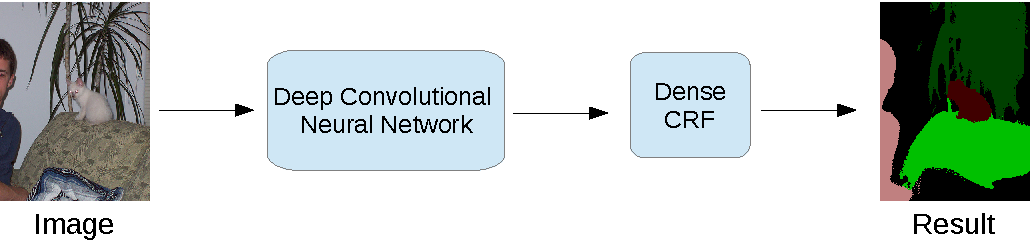
\includegraphics[width=0.9\linewidth]{fig/model_test.pdf} 
  \caption{Overview of the DeepLab-CRF model.}
  \label{fig:model_test}
\end{figure}

\subsection{Model Training Using Fully Annotated Images}
\label{sec:train_pixel}

The network parameters $\thetav$ are trained by stochastic gradient
descent (SGD) so as to minimize the average log-loss 
\begin{equation}
  \label{eq:log_loss}
  L(\thetav) = \frac{1}{N} \sum_{i = 1}^N \log P_i(l_i; \thetav)
\end{equation}
between the model predictions and the pixel-wise ground truth
labels $\{l_i\}_{i = 1}^N$, as illustrated in
Figure~\ref{fig:model_train_pixel}. Similarly to
\citet{chen2014semantic}, we do not include the Dense CRF module into
the training pipeline for simplicity and speed during training.

Learning the DeepLab-CRF model on fully annotated images works very
well in practice, yielding state-of-art performance (66.4\% IOU) in
the challenging PASCAL VOC 2012 image segmentation benchmark. However,
the need for such detailed annotations makes it harder to gather very
large training datasets and makes it difficult to train the model
for new domains, especially when the number of candidate labels
(\ie, the cardinality of the label set $\mathcal{L}$) is large.

\begin{figure}[htbp!]
  \centering
  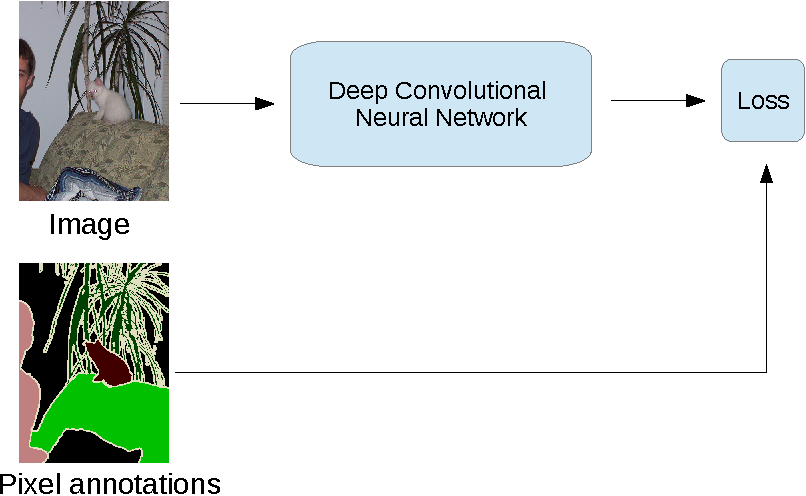
\includegraphics[width=0.9\linewidth]{fig/model_train_pixel.pdf} 
  \caption{DeepLab model training from fully annotated images.}
  \label{fig:model_train_pixel}
\end{figure}

\subsection{Model Training Using Bounding Box Weak Annotations}
\label{sec:train_bbox}

Collecting bounding box annotations is significantly easier compared
to pixel-level ground truth segmentations. We have explored two
alternative methods for training the DeepLab segmentation model from
bounding boxes with object-level labels. In both methods we estimate
dense segmentation maps from the bounding box annotation as a
pre-processing step, then employ the training procedure of
\secref{sec:train_pixel} treating these estimated labels as
ground-truth, as illustrated in \figref{fig:model_train_bbox}.

\begin{figure}[htbp!]
  \centering
  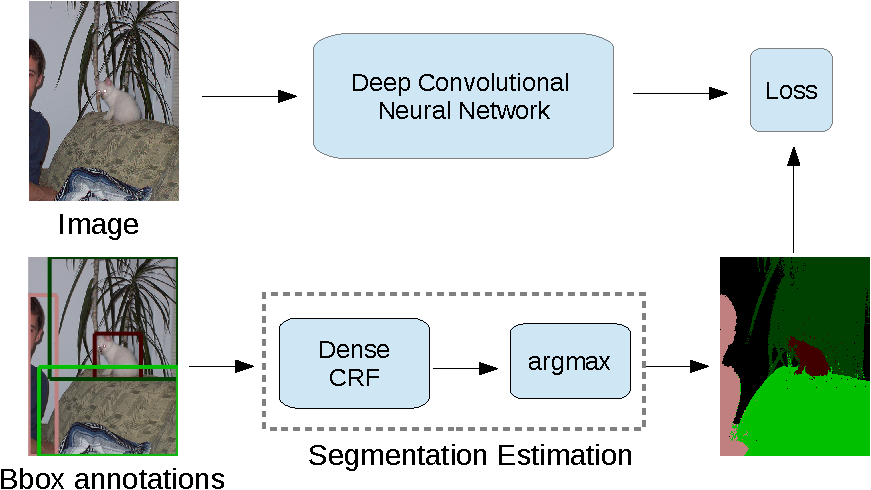
\includegraphics[width=0.9\linewidth]{fig/model_train_bbox.pdf} 
  \caption{DeepLab model training using bounding box data and
    automated foreground/ background segmentation.}
  \label{fig:model_train_bbox}
\end{figure}

The first \textsl{Bbox-Baseline} method amounts to simply considering
each pixel within the bounding box as positive example for the
respective object class. Ambiguities are resolved by assigning pixels
that belong to multiple bounding boxes to the one that has the
smallest area.

The bounding boxes fully surround objects but also contain background
pixels that contaminate the training set with false positive examples
for the respective object classes. To discard these background pixels,
we have also explored a second \textsl{Bbox-Seg} method in which we
perform automatic foreground/background segmentation in the spirit of
\citet{rother2004grabcut}. We assign to pixels in the foreground
segment the label of the bounding box and to pixels in the background 
segment the background label. For the foreground/background
segmentation we employ once more the Dense CRF model. More
specifically, we constrain the center area of the bounding box ($K\%$
of pixels within the box) to be foreground, while we constrain pixels
outside the bounding box to be background. We implement this by
appropriately setting the unary terms of \equref{eq:fully_crf}. The
Dense CRF is then applied to infer the label for pixels in between. We
cross-validate the Dense CRF parameters so as to maximize segmentation
accuracy in a small held-out set of fully-annotated images.

Examples of estimated segmentations with the two methods are
shown in \figref{fig:bbox_illustration}.

\begin{figure}
  \centering
  \begin{tabular}{c c c c}
    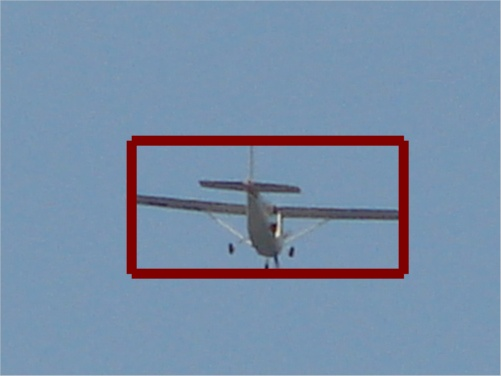
\includegraphics[width=0.21\linewidth]{fig/erode_bbox/img/2010_004063.jpg} & 
    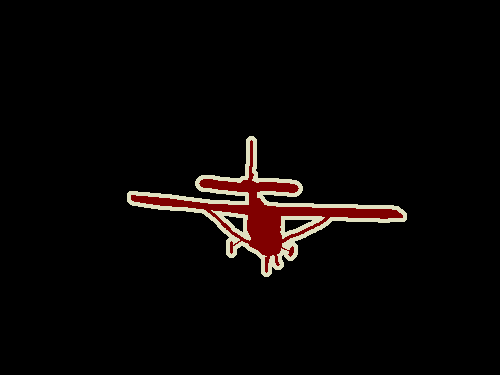
\includegraphics[width=0.21\linewidth]{fig/erode_bbox/gt/2010_004063.png} & 
    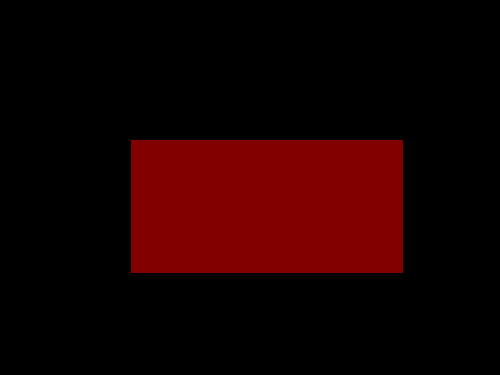
\includegraphics[width=0.21\linewidth]{fig/erode_bbox/bbox/2010_004063.png} & 
    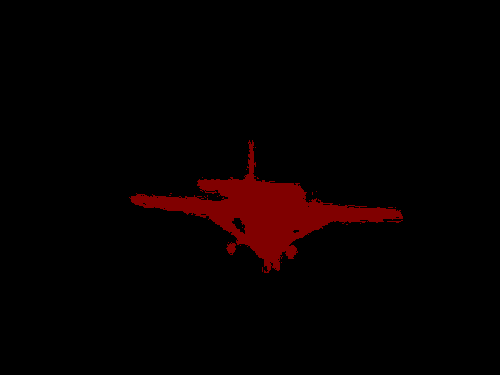
\includegraphics[width=0.21\linewidth]{fig/erode_bbox/crf/2010_004063.png} \\    
    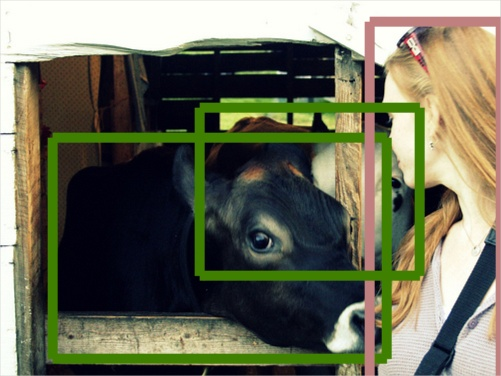
\includegraphics[width=0.21\linewidth]{fig/erode_bbox/img/2009_000219.jpg} & 
    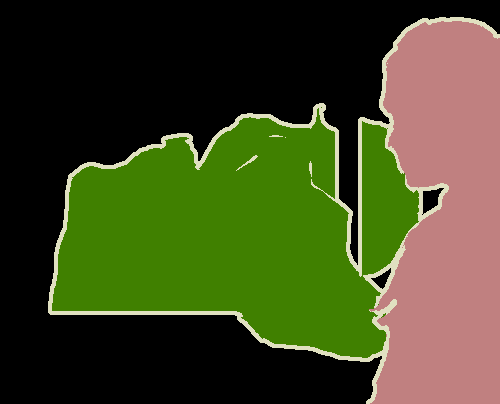
\includegraphics[width=0.21\linewidth]{fig/erode_bbox/gt/2009_000219.png} & 
    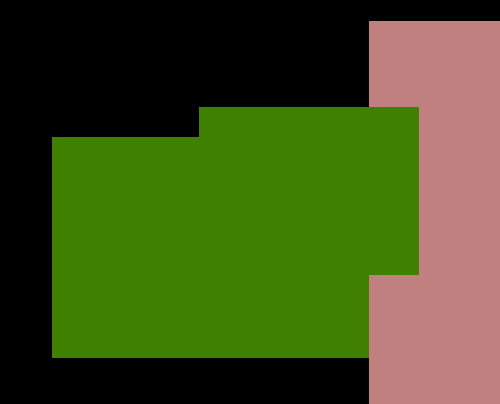
\includegraphics[width=0.21\linewidth]{fig/erode_bbox/bbox/2009_000219.png} & 
    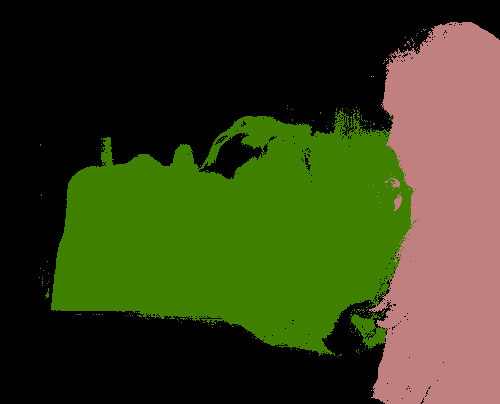
\includegraphics[width=0.21\linewidth]{fig/erode_bbox/crf/2009_000219.png} \\        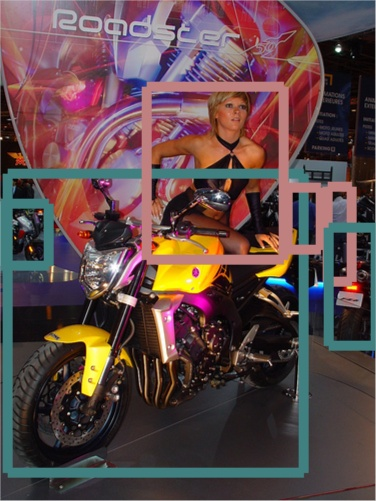
\includegraphics[width=0.21\linewidth]{fig/erode_bbox/img/2009_002382.jpg} & 
    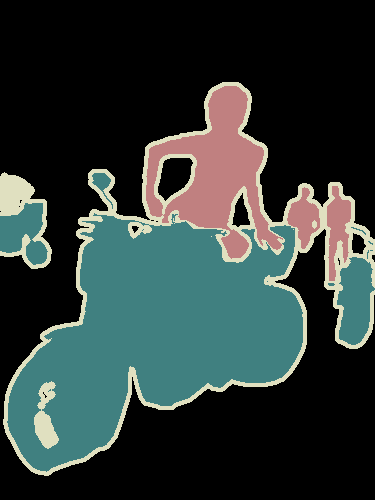
\includegraphics[width=0.21\linewidth]{fig/erode_bbox/gt/2009_002382.png} & 
    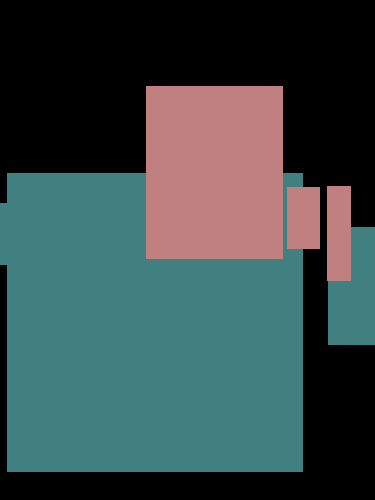
\includegraphics[width=0.21\linewidth]{fig/erode_bbox/bbox/2009_002382.png} & 
    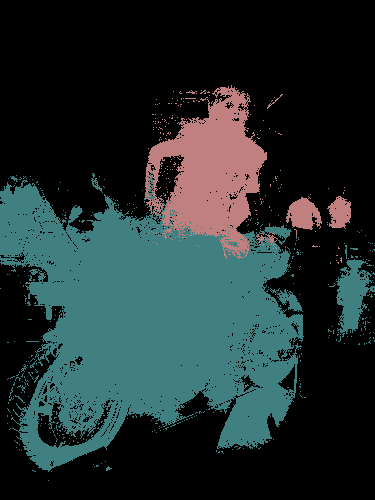
\includegraphics[width=0.21\linewidth]{fig/erode_bbox/crf/2009_002382.png} \\    
    {\scriptsize Image with Bbox} & {\scriptsize Ground-Truth} & {\scriptsize Bbox-Baseline} & {\scriptsize Bbox-Seg}
  \end{tabular}
  \caption{Segmentation estimation for bounding box annotations. We
    show three examples from easy to hard.}
  \label{fig:bbox_illustration}
\end{figure}


\subsection{Model Training Using Weak Image-Level Labels}
\label{sec:train_image}

Training the DeepLab segmentation model using only image-level labels
is significantly more challenging.

\paragraph{Previous MIL Approaches and their Limitations}

Previous related CNN literature employs multiple instance learning
variants to address the weak supervision problem, but has demonstrated
limited success in learning accurate segmentation models. 

In particular, recent work by \citet{pathak2014fully} attempts to
learn the CNN parameters for the segmentation model by adapting an MIL
formulation previously employed for image classification tasks
\citep{oquab2014weakly, papandreou2014untangling}. More specifically,
during training they compute an aggregate image-level response for
each class $x$ as the maximum class score across all pixel positions
$i$
\begin{equation}
  \label{eq:mil}
  \bar{f}(x; \thetav) = \max_i f_i(x; \thetav) \,
  \quad \mathrm{and} \quad
  \bar{P}(x; \thetav) \propto \exp \left( \bar{f}(x; \thetav) \right)
\end{equation}
which is then combined with the image-level ground-truth label $l$ to
compute the whole-image loss $\bar{L}(\thetav) = \log \bar{P}(l;
\thetav)$. A similar formulation with softmax instead of max
aggregation has been pursued before by \citet{pinheiro2014weakly}.

There are several limitations to this MIL-based approach to the image
segmentation problem. \emph{First}, the model does not explicitly
encourage good localization during training, since it suffices to give
strong response for the correct class anywhere within the
image. \emph{Second}, MIL does not promote good
object coverage. For example, it is often sufficient to learn a good
face detector to reliably determine whether an image contains a
person. However, this face detector will give false-negative
responses on the rest of the human body and is thus not appropriate
for segmenting whole persons. \emph{Third}, this MIL formulation
does not incorporate competition across channels, with maximum
responses of multiple classes potentially coming from the same image
position. The model is thus allowed to ignore a large portion of the
image content during training.
%% \emph{Third}, network back-propagation
%% only activates a single path per label through the maximally
%% responding pixel position ignoring a large portion of the image
%% content, thus slowing down training.
These issues have severely undermined the success of previous CNN/MIL
approaches to image segmentation and the performance of such models
trained on weak labels significantly lags their counterparts trained
on pixel-level annotations, as explained in \secref{sec:experiments}.

\paragraph{Weakly Supervised Expectation-Maximization}

We propose an alternative training procedure based on a modified
Expectation-Maximization (EM) algorithm adapted to our weakly-labeled
image segmentation setting.

In this setting, we consider the pixel-level semantic labels
$\{l_i\}_{i=1}^N$ as latent variables. We incorporate the image-level
semantic labels as side-information that biases the E-step of the EM
algorithm, as detailed in Algorithm~\ref{algo:em_fixed_bias} and
illustrated in \figref{fig:model_train_image}. The positive
foreground and background biases $c_f$ and $c_b$ favor the score maps
corresponding to labels present in the image, incorporating the prior
information carried by the image-level weak annotation. A similar
approach has been employed before by \citet{Lu2013sports}. We have
obtained better results by choosing $c_f > c_b$, slightly favoring
foreground objects over the background to encourage higher foreground
object coverage. Notably, the E-step assigns a label to every image
pixel and thus the model parameters are updated during the M-step to
better explain the whole image content.

\begin{algorithm}[!htbp]
  \centering
  \begin{algorithmic}[1]
    \algrenewcommand\algorithmicrequire{\textbf{Input:}}
    \Require CNN parameters $\thetav$ and biases $c_f, c_b > 0$.
    \algrenewcommand\algorithmicrequire{\textbf{E-Step:}}
    \Require For each image position $i$
    \State $\hat{f}_i (x_i; \thetav) = f_i(x_i; \thetav) + c_f$, if $x_i$ is FG label \Comment{FG bias}
    \State $\hat{f}_i (x_i; \thetav) = f_i(x_i; \thetav) + c_b$, if $x_i$ is BG label \Comment{BG bias}
    \State $\hat{f}_i (x_i; \thetav) = f_i(x_i; \thetav)$, if label $x_i$ not present
    \State $\hat{l}_i = \argmax_{x_i \in \mathcal{L}} \hat{f}_i (x_i; \thetav)$ \Comment{Hard assignments}
    \algrenewcommand\algorithmicrequire{\textbf{M-Step:}}
    \Require
    \State $\hat{L}(\thetav) = \frac{1}{N} \sum_{i = 1}^N \log P_i(\hat{l}_i; \thetav)$ \Comment{Expected loss}
    \State Update $\thetav$ by SGD with momentum on $\hat{L}(\thetav)$
    \end{algorithmic}
  \caption{Weakly-Supervised EM (fixed bias version)}
  \label{algo:em_fixed_bias}
\end{algorithm}

\begin{figure}[htbp!]
  \centering
  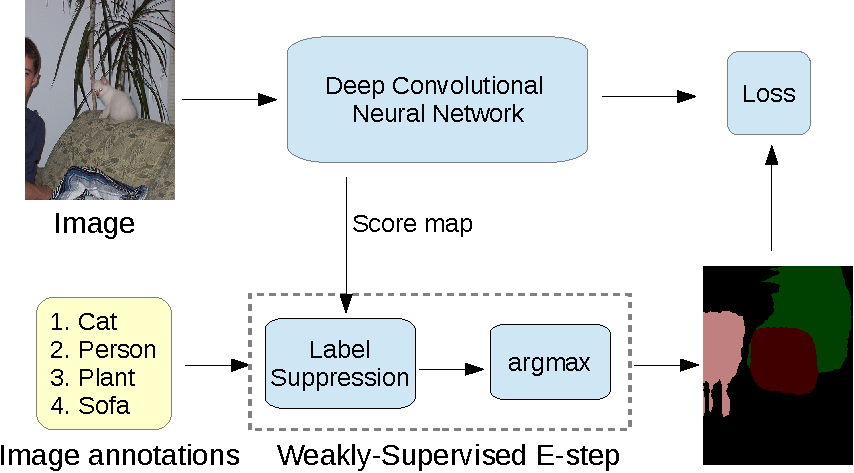
\includegraphics[width=0.9\linewidth]{fig/model_train_image.pdf} 
  \caption{DeepLab model training using image-level labels by
    weakly-supervised Expectation-Maximization.}
  \label{fig:model_train_image}
\end{figure}

We have also experimented with an adaptive variant of
Algorithm~\ref{algo:em_fixed_bias} in which the biases are chosen
adaptively per image so as a pre-defined proportion of the image area
is assigned to the foreground object class, similarly to
\citet{kuck2005individuals}. This acts as a hard constraint that
explicitly prevents the background score from prevailing in the whole
image, also promoting higher foreground object coverage. As reported
in the experimental section, we have found this adaptive variant to
perform better in the purely weakly supervised scenario, whereas the
fixed bias variant works best in the semi-supervised training scenario
discussed next.

\subsection{Semi-Supervised Model Training Using Both Fully and Weakly Annotated Images}
\label{sec:train_semi}

In practice, we often have access to a large number of weakly
image-level annotated images and can only afford to procure detailed
pixel-level annotations for a small fraction of these images. We
propose to handle this hybrid semi-supervised training scenario by
combining the methods presented in the previous sections, as
illustrated in Figure~\ref{fig:model_illustrations_twoEnd}. In SGD
training of our deep CNN models, we bundle to each mini-batch a fixed
proportion of strongly/weakly annotated images, and employ the
fixed-bias version of our weakly-supervised EM algorithm in estimating
at each iteration the latent semantic segmentations for the weakly
annotated images. We demonstrate in \secref{sec:experiments} that one
needs to annotate in detail at the pixel-level only a small part of
the dataset and use image-level labels for the remaining part to
achieve the same level of performance with a DeepLab model trained
with the whole dataset fully annotated.

\begin{figure}[htbp!]
  \centering
  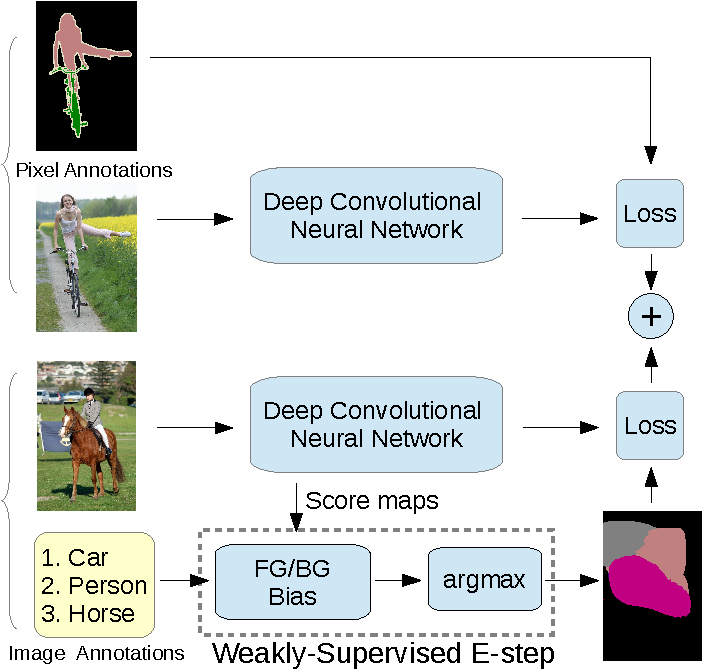
\includegraphics[width=0.9\linewidth]{fig/model_train_twoEnd.pdf} 
  \caption{DeepLab model training on a union of full (strong labels) 
    and image-level (weak labels) annotations.}
  \label{fig:model_illustrations_twoEnd}
\end{figure}


 %%% Local Variables:
 %%% mode: latex
 %%% TeX-master: "top.tex"
 %%% End:
